\usetikzlibrary{arrows.meta,calc}
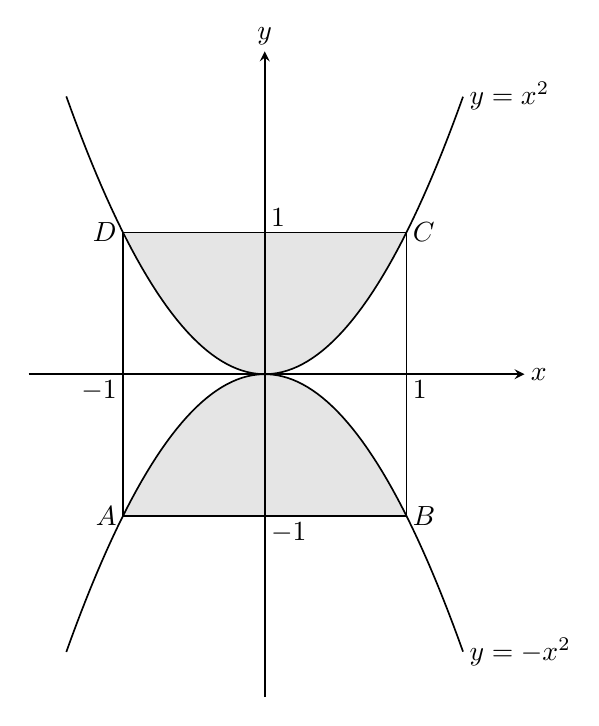
\begin{tikzpicture}[x=1cm,y=1cm,line width=.6pt,>=stealth]
\fill[gray!20] (-1.8,1.8)--(1.8,1.8)--plot[domain=1.8:-1.8,samples=60] (\x,{\x*\x/1.8})--cycle;
\fill[gray!20] (-1.8,-1.8)--(1.8,-1.8)--plot[domain=1.8:-1.8,samples=60] (\x,{-\x*\x/1.8})--cycle;
\draw[->] (-3.0,0)--(3.3,0) node[right,inner sep=0pt,xshift=2pt] {$x$};
\draw[->] (0,-4.1)--(0,4.1) node[above,inner sep=0pt,yshift=2pt] {$y$};
\draw (-1.8,-1.8) rectangle (1.8,1.8);
\draw[domain=-1.4:1.4,samples=80] plot ({1.8*\x},{1.8*\x*\x});
\draw[domain=-1.4:1.4,samples=80] plot ({1.8*\x},{-1.8*\x*\x});
\node[left,inner sep=0pt,xshift=-2pt] at (-1.8,1.8) {$D$};
\node[right,inner sep=0pt,xshift=2pt] at (1.8,1.8) {$C$};
\node[left,inner sep=0pt,xshift=-2pt] at (-1.8,-1.8) {$A$};
\node[right,inner sep=0pt,xshift=2pt] at (1.8,-1.8) {$B$};
\node[below left,inner sep=0pt,xshift=-2pt,yshift=-2pt] at (-1.8,0) {$-1$};
\node[below right,inner sep=0pt,xshift=2pt,yshift=-2pt] at (1.8,0) {$1$};
\node[above right,inner sep=0pt,xshift=2pt,yshift=2pt] at (0,1.8) {$1$};
\node[below right,inner sep=0pt,xshift=2pt,yshift=-2pt] at (0,-1.8) {$-1$};
\node[right,inner sep=0pt,xshift=2pt] at (2.52,3.528) {$y=x^{2}$};
\node[right,inner sep=0pt,xshift=2pt] at (2.52,-3.528) {$y=-x^{2}$};
\end{tikzpicture}
